\documentclass[specialist, twoside,
substylefile = spbu.rtx,
               subf,href,colorlinks=true, 12pt]{disser}

\usepackage[a4paper,
            mag=1000, includefoot,
            left=3cm, right=1.5cm, top=2cm, bottom=2cm, headsep=1cm, footskip=1cm
            % margin=0.1cm
            ]{geometry}
\usepackage[T2A]{fontenc}
\usepackage[utf8]{inputenc}
\usepackage[english,russian]{babel}
\ifpdf\usepackage{epstopdf}\fi

% Использовать полужирное начертание для векторов
\let\vec=\mathbf

% Включать подсекции в оглавление
\setcounter{tocdepth}{2}

\usepackage[defaultmono]{droidmono}
\usepackage[T2A]{fontenc}
% \usepackage{csquotes}

\usepackage[intlimits]{amsmath}
\usepackage{amsfonts}
\usepackage{amssymb}
\usepackage{amsthm}
\usepackage{mathtools}
\usepackage{nicefrac}

\usepackage{algorithm2e}
\usepackage{graphicx}
\graphicspath{ {media/} }
\usepackage{listings}
\usepackage{color}

\usepackage[fixlanguage]{babelbib}
\selectbiblanguage{russian}

% \usepackage{natbib}
% \usepackage[style=numeric]{biblatex}
% \addbibresource{biblio-u.bib}

\usepackage{hyperref}
\newtheorem{theorem}{Теорема}
\newcommand{\ev}{\mathsf{E}}
\newcommand{\vfi}{\varphi}
\newcommand{\prob}[1]{\mathsf{P}\left(#1\right)}
\newcommand{\R}{\ensuremath{\mathbb{R}}}
\newcommand{\Tau}{\ensuremath{\mathfrak{T}}}
\newcommand{\GothB}{\mathfrak{B}}
\newcommand{\norm}[1]{\left\lVert#1\right\rVert}
\newcommand{\Vhat}{\hat{V}}
\newcommand{\vhat}{\hat{v}}
\newcommand{\maxset}[1]{\max\left\lbrace#1\right\rbrace}
\DeclareMathOperator*{\argmax}{arg\,max}
\DeclareMathOperator*{\argmin}{arg\,min}


\setlength\parindent{0pt}
\setlength\parskip{0.4em}

\lstdefinestyle{customjava}{
%   belowcaptionskip=1\baselineskip,
  	breaklines=true,
  	breakatwhitespace=true,
%   xleftmargin=\parindent,
%   language=Java,
%   showstringspaces=false,
   	basicstyle=\footnotesize\fdmfamily,
   	keywordstyle=\bfseries\color{blue},
  	commentstyle=\color{magenta},
  	morekeywords={ImitatedAsset, },
  	% identifierstyle=\color{green},
%   stringstyle=\color{orange},
}
\lstset{style=customjava, language=Java}

\usepackage{tikz}
\usetikzlibrary{arrows}
\usetikzlibrary{positioning}
\usetikzlibrary{graphs}

%----------------------------------------------------------------
\begin{document}

\institution{%
    Правительство Российской Федерации \\
    Федеральное государственное бюджетное образовательное учреждение \\
    высшего профессионального образования \\
    «Санкт-Петербургский государственный университет» \\
    Кафедра статистического моделирования
}

% Имя лица, допускающего к защите (зав. кафедрой)
\apname{д.\,ф.-м.\,н., профессор С.\,М.~Ермаков}

\title{Бакалаврская работа}

% Тема
\topic{\normalfont\scshape%
    Имитационная модель американских опционов}

% Автор
\author{Миллер Анастасия Александровна}

% Научный руководитель
\sa       {С.\,М.~Ермаков}
\sastatus {д.\,ф.-м.\,н., профессор}

% Рецензент
\rev      {Т.\,М.~Товстик}
\revstatus{к.ф.-м.н., доцент}

% Город и год
\city{Санкт-Петербург}
\date{\number\year}

\maketitle

%%
%% Titlepage in English
%%
%
\institution{%
    Saint Petersburg State University \\
    Department of Statistical Modelling
}
%
%% Approved by
\apname{Professor S.\,M.~Ermakov}
%
\title{Bachelor's Thesis}
%
%% Topic
\topic{\normalfont\scshape %
    Simulation model of American options}
%
%% Author
\author{Miller Anastasiia} % Full Name
%
%% Scientific Advisor
\sa       {S.\,M.~Ermakov}
\sastatus {Doctor of Physics and Mathematics, Professor}
%
%% Reviewer
\rev      {T.\,M.~Tovstik}
\revstatus{Candidate of Physics and Mathematics, Associate Professor}
%
%% City & Year
\city{Saint Petersburg}
\date{\number\year}
%
\maketitle[en]

\tableofcontents
\intro
Работа посвящена некоторым методам оценки стоимости Американских опционов. Опцион --- один из производных финансовых инструментов (вместе с фьючерсами, свопами, контрактами на разницу цен), активно использующихся на современных финансовых рынках. Интерес представляет оценивание <<справедливой>> цены опциона.

Более подробно, \emph{опцион} --- договор, по которому покупатель опциона (потенциальный покупатель или потенциальный продавец базового актива — товара, ценной бумаги) получает право, но не обязательство, совершить покупку или продажу данного актива (\emph{исполнить} опцион) по заранее оговорённой цене (\emph{цене страйк}) в определённый договором момент в будущем или на протяжении определённого отрезка времени. При этом продавец опциона несёт обязательство совершить ответную продажу или покупку актива в соответствии с условиями проданного опциона. Различают опционы на продажу актива и на его покупку. По количеству и типу моментов времени, в которые можно совершить оговорённую в контракте сделку, опционы подразделяются на Европейские (совершить сделку можно только в один указанный момент времени) и Американские (совершить сделку можно в любое время вплоть до указанного), а также более экзотические варианты (например, Бермудский, позволяющий совершить сделку в один из нескольких указанных моментов).

Опционный контракт предполагает возможность смены владельца, а исполнение опциона (совершение покупки или продажи, право на которую даётся в контракте) может принести выгоду по сравнению с аналогичной операцией на рынке, поэтому опционный контракт имеет собственную цену. Значение этой цены неочевидно, так как невозможно точно предсказать размер прибыли, которую получит владелец контракта.

Целью работы является анализ и упрощение (вычислительное) некоторых методов оценки стоимости Американских опционов.

\chapter{Имитационные модели оценки американского опциона}

Традиционный подход предполагает следование гипотезе эффективного рынка, которая влечёт определение <<справедливой>> цены опциона как \emph{такой цены, при которой ни продавец, ни покупатель в среднем не получают прибыли}. Тогда ценой Американского опциона является математическое ожидание прибыли, полученной при исполнении опциона в оптимальный момент времени, а задача оценки оказывается частным случаем проблемы остановки выбора (подробнее о проблеме с этой точки зрения можно посмотреть в \cite{Peskir2006}, там же сформулировано дифференциальное уравнение для цены Американского опциона).

Опцион определяется своим временем жизни $[0;T]$, базовым активом $X$ (под $X(t)$ будем подразумевать состояние актива в момент времени $t$, являющееся случайной величиной, $S(t) = S(X(t))$ --- цену базового актива в момент $t$), на который выписан опцион (список возможных активов на территории Российской Федерации представлен в \cite{fsfr}), процессом $U(t), t\in [0;T]$, представляющим дисконтированное значение функции выплат (разницы между рыночной стоимостью базового актива и ценой страйк, оговорённой в контракте; значение функции выплат показывает выгоду, получаемую владельцем опциона при исполнении), и множеством $\Tau$ моментов времени, в которых возможно исполнить опцион. Тогда задача состоит в нахождении 
\begin{equation}\label{eq:supremum_of_expectation}
	\sup_{\tau\in\Tau} \ev U(\tau)
\end{equation}
(формальное обоснование того, почему это выражение может быть названо ценой опциона, есть в \cite{Duffie2001}).

Мы будем действовать в менее общей постановке задачи, в предположении, что вся необходимая информация о состоянии базового актива в момент времени $t$ содержится в переменной $X(t)\in \mathfrak{R}^d$ и $X(t)$ является марковским процессом. Дисконтированное значение функции выплат обозначается $h\left(X\left(t\right)\right) \geq 0 \quad\forall t\in \left[0;T\right]$, и тогда формулировка задачи сводится к оцениванию $$\sup_{\tau\in\Tau}\ev h\left(X\left(\tau\right)\right).$$

В случае классического Американского опциона пут (право на продажу актива по фиксированной цене $K$) $h(t) = e^{-rt}\left(K-S\left(t\right)\right)^+$, опциона колл (право на покупку актива по фиксированной цене $K$) --- $h(t) = e^{-rt}\left(S\left(t\right) - K\right)^+$, где $e^{-rt}$ --- дисконтирующий множитель для процентной ставки в непрерывным начислением процентов $r$, обеспечивающий измерение цен в одних и тех же единицах.

Для решения задачи об оценивании Европейского опциона применимы формулы Блэка-Шоулса (при достаточно сильных предположениях о поведении базового актива и влиянии его на цену производного финансового инструмента). В случае же Американского опциона граница исполнения (та цена базового актива $\bar{S}(t)$, при которой досрочное исполнение становится оптимальным) априори неизвестна, что делает решение уравнения невозможным (см. \cite{Lyuu2007} и ссылки оттуда, \cite{Peskir2006}). Поэтому для построения оценок Американского опциона используются различные имитационные методы. Все они на стадии теоретического или практического воплощения предполагают, что опцион может быть исполнен лишь в некоторые моменты времени $0 = t_0 < t_1 < \cdots < t_{m-1} < t_m=T$ (такой опцион иногда называют Бермудским, имея в виду его расположенность между Европейской и Американской моделью исполнения; такого вида финансовые инструменты действительно существуют, например, дискретизация может быть обусловлена наличием информации о том, что исполнение опциона может быть оптимальным только в эти моменты времени).  Здесь и далее будем обозначать $X_i = X\left(t_i\right)$, $S_i = S\left(X_i\right)$.

Имея дискретизацию $t_0, t_1, \ldots, t_m$, мы можем выразить цену опциона как решение $V_0\left(X_0\right)$ следующей задачи динамического программирования:
\begin{equation}\label{eq:common_recursive_statement}
	\begin{aligned}
		V_m\left(x\right) &= h_m\left(x\right) \\
		V_k\left(x\right) &= \max\left\lbrace h_k\left(x\right), \ev\left(V_{k+1}\left(X_{k+1}\right)\middle\vert X_k = x\right)\right\rbrace, k\in 0\mathrel{:}m-1
	\end{aligned}
\end{equation}

Обзор методов, использующих дискретизацию пространства состояний и имитирующих поведение базового актива, представлен ниже.

\paragraph{Биномиальные и триномиальные деревья}
Использование биномиальных и триномиальных деревьев предполагает существенное ограничение множества состояний, в которых может оказаться базовый актив в течение $[0;T]$. Предполагается, что за каждый отрезок времени $\left[t_{k-1};t_k\right], k\in 1:m$ цена базового актива $S$ может измениться (в биномиальной модели) лишь двумя способами: превратиться в $Su$ с вероятностью $p_u$ и превратиться в $Sd$ с вероятностью $p_d=1$. В триномиальной модели добавляется вероятность того, что цена актива не изменится, а на значения скачков цены накладывается ораничение $ud = 1$. В обоих случаях предположение сразу сужает класс опционов до тех, у которых базовый актив состоит лишь из одного вида товаров. Результатом модели становится дерево состояний актива, представленное на рис. \ref{fig:trinomial_tree}. В силу предположения о дискретности процесса изменения состояния актива $\ev\left(V_{k+1}\left(X_{k+1}\right)\middle\vert X_k = x\right)$ может быть подсчитано точно, и, обходя построенное дерево в глубину, мы получаем значение стоимости опциона.

\begin{figure}
\centering
\begin{tikzpicture}[->,>=stealth',shorten >=1pt,auto,rectangle,draw]
	\matrix[row sep=10mm,column sep=0.05\linewidth] {
		% 				 & 					 & 					   & \node (3111) {$Suuu$}; \\
		% 				 & 					 & \node (211) {$Suu$}; & \node (311) {$Su$}; \\
		% 				 & \node (11) {$Su$};& \node (21) {$Su$};  & \node (31) {$Su$}; \\
		% \node (0) {$S$}; & \node (10) {$S$}; & \node (20) {$S$};   & \node (30) {$S$}; \\
		% 				 & \node (12) {$Sd$};& \node (22) {$Sd$};  & \node (32) {$Sd$};  \\
		% 				 & 					 & \node (222) {$Sdd$};& \node (322) {$Sdd$}; \\
		% 				 & 					 & 					   & \node (3222) {$Sddd$}; \\
        &&&\node (0) {$S$};&&&\\
        &&\node (11) {$Su$};&\node (10) {$S$};&\node (12) {$Sd$};&& \\
        &\node (211) {$Suu$};&\node (21) {$Su$};&\node (20) {$S$};&\node (22) {$Sd$};&\node (222) {$Sdd$};& \\
        \node (3111) {$Suuu$};&\node (311) {$Su$};&\node (31) {$Su$};&\node (30) {$S$};&\node (32) {$Sd$};&\node (322) {$Sdd$};&\node (3222) {$Sddd$};  \\
    };
    \path 	(0)	edge[->]	(11)
    			edge[->]	(10)
    			edge[->]	(12)
    		(11)	edge[->]	(211)
    				edge[->]	(21)
    				edge[->]	(20)
    		(10)	edge[->]	(21)
    				edge[->]	(20)
    				edge[->]	(22)
    		(12)	edge[->]	(20)
    				edge[->]	(22)
    				edge[->]	(222)
    		(211)	edge[->]	(3111)
    				edge[->]	(311)
    				edge[->]	(31)
    		(21)	edge[->]	(311)
    				edge[->]	(31)
    				edge[->]	(30)
    		(20)	edge[->]	(31)
    				edge[->]	(30)
    				edge[->]	(32)
    		(22)	edge[->]	(30)
    				edge[->]	(32)
    				edge[->]	(322)
    		(222)	edge[->]	(32)
    				edge[->]	(322)
    				edge[->]	(3222);
\end{tikzpicture}

\caption{Триномиальное дерево}
\label{fig:trinomial_tree}
\end{figure}

Модель хороша линейно растущим при увеличении $m$ числом вершин, но существенно ограничивает множество состояний опциона, порождая этим неточность.

\paragraph{Дискретизация пространства состояний}
Развивая идею об ограничении множества состояний, мы можем ограничить множество состояний, в которых может оказаться базовый актив в данный момент времени, некоторым набором $A_{i1}, \ldots, A_{ib_i}$ (или, что аналогично, разбить множество состояний на подмножества $A_{ij}$), для $i=0 \;\;b_i = 1$ и $A_0 = \left\lbrace X_0\right\rbrace$. Тогда мы можем определить вероятности $$p^i_{jk} = \prob{X_{i+1}\in A_{i+1, k} \middle\vert X_i\in A_{ij}}, i\in 1:m, j\in 1:b_i, k\in 1:b_{i+1}.$$

Если нам известны эти вероятности и значение функции выплат для каждого из множеств состояний, то мы можем точно посчитать значение $V_0\left(X_0\right)$ по формуле \eqref{eq:common_recursive_statement}. В случае, когда эти вероятности неизвестны (а они вряд ли известны), стоит воспользоваться их выборочной оценкой, полученной методом Монте-Карло. Для получения таких оценок достаточно зафиксировать набор состояний $\left\lbrace A_{i1}, \ldots, A_{ib_i}\right\rbrace_{i=1}^m$ и промоделировать достаточно много траекторий изменения состояния актива на промежутке $\left[0;T\right]$. Для определения значения функции выплат $h_{ij}, i \in 1:m, j\in 1:b_i$ можно также воспользоваться многократным моделированием и определить $h_{ij}$ как $\ev\left( h_i(x)\middle\vert x\in A_{ij}\right)$. Ключевым вопросом в этом методе остаётся выбор множества состояний.

\paragraph{Параметрические приближения}
Возвращаясь к формулировке \eqref{eq:supremum_of_expectation}, мы можем ограничить не пространство состояний, а пространство стратегий принятия решения об исполнении опциона. Идея может быть хорошо проиллюстрирована на одномерных активах (состоящих из одного вида товаров). На рис. \ref{fig:excercise_boundary} мы видим, как выглядит пример области исполнения --- области, при попадании состояния базового актива в которую оптимальным решением будет исполнить опцион. Задача переформулируется в виде нахождения
$$\sup_{\theta \in \Theta} \ev h_{\tau(\theta)}\left(X_{\tau\left(\theta\right)}\right),$$ 
где $\tau\left(\theta\right)$ --- момент времени, параметризованный по $\theta$. Имея множество $\Theta$, мы можем найти оценку супремума, находя значение параметра, доставляющее максимум выборочному математическому ожиданию по смоделированным траекториям.

Основная проблема заключается здесь в том, что оптимальная в семействе стратегия не обязана быть оптимальной на множестве всех стратегий.
\begin{figure}[htb]
\centering
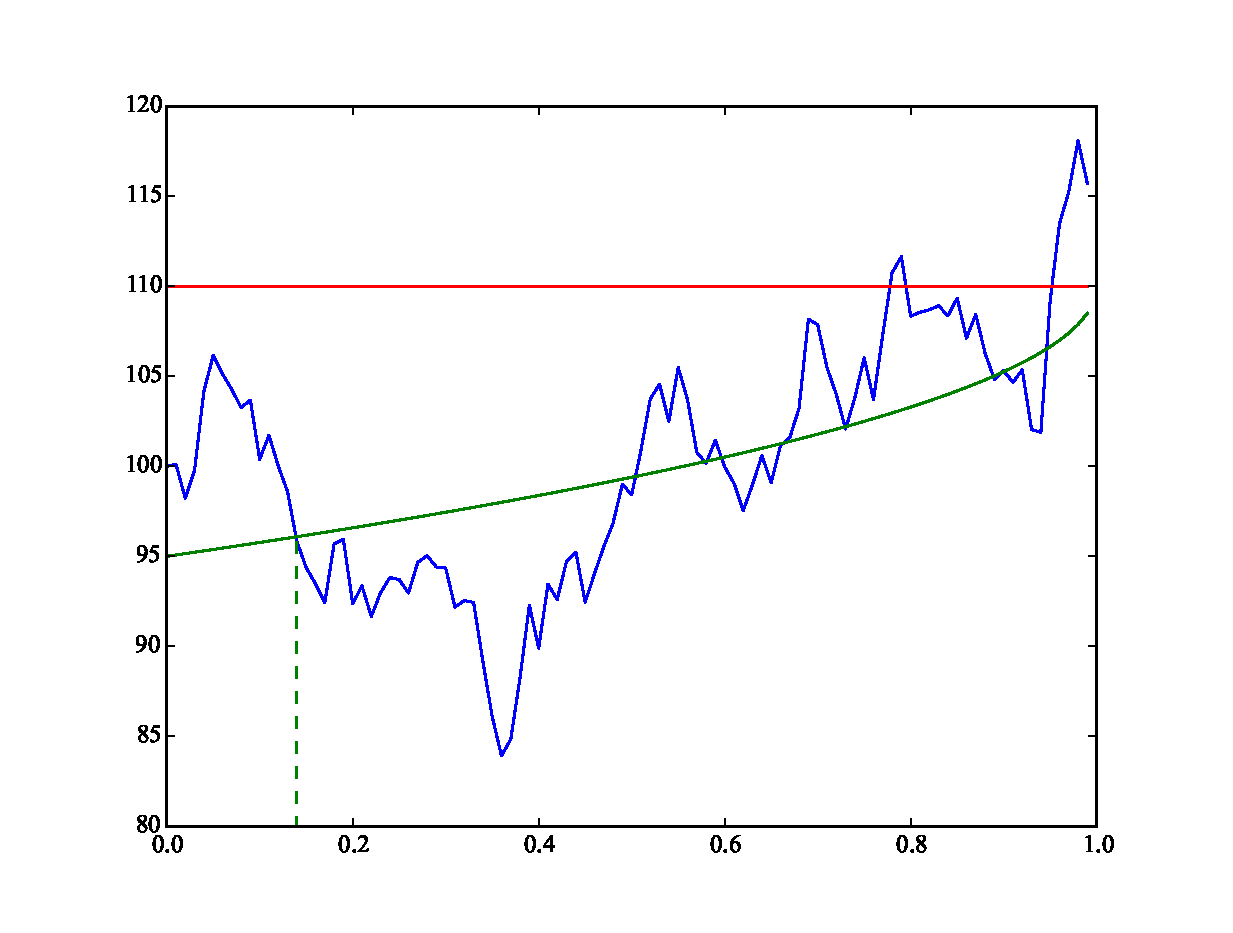
\includegraphics[width=0.7\textwidth]{random_process_with_excercise_boundary}
\caption{Граница исполнения для Американского опциона пут с функцией выплат $\left(K-S(t)\right)^+$ (форма границы --- примерная, точная форма неизвестна). Опцион исполняется, как только цена актива впервые достигает границы. Горизонтальная линия --- цена страйк опционного контракта. Пунктирной линией отмечен момент оптимального исполнения опциона.}
\label{fig:excercise_boundary}
\end{figure}

\paragraph{Метод стохастической сетки}
Метод стохастической сетки решает задачу динамического программирования \eqref{eq:common_recursive_statement} с помощью генерирования случайных траекторий состояния базового актива. Сетку, получающуюся при назначении всех вершин предыдущего поколения родительскими вершинами для всех вершин следующего поколения, можно увидеть на рис. \ref{fig:stohastic_mesh}.
\begin{figure}[htpb]
\centering
\includegraphics[width=0.7\textwidth]{stohastic_mesh_vector}
\caption{Сетка состояний базового актива при использовании метода стохастической сетки}
\label{fig:stohastic_mesh}
\end{figure}

Количество узлов в сетке ограничено $mn$, где $m$ ---  число дат исполнения опциона, $n$ --- число промоделированных траекторий. Неоднозначным остаётся лишь выбор весов, присвиваемых дугам сетки.

Все вышеописанные методы подробно рассмотрены в \cite{Glasserman2004}.

Также существуют некоторые аналитические формы приближённых оценок стоимости Американского опциона (см. \cite{Haug2007}, глава 3, и последующие ссылки), но они накладывают более жёсткие ограничения на сущность базового актива.

В следующей главе подробно рассматривается ещё один имитационный метод оценки: метод случайных деревьев, являющийся объектом исследования этой работы. Обладая некоторыми существенными недостатками, он, тем не менее, представляет интерес для исследования из-за потенциальной возможности обощения на более широкий класс задач.

\chapter{Метод случайных деревьев}

Метод случайных деревьев, предложенный в \cite{Broadie1997}, ищет решение проблемы оптимального времени остановки и оценивает истинное значение цены Американского опциона (в отличие от метода параметрических приближений).

\par Вместо того, чтобы строить оценку, каким-либо образом стремящуюся к $V_0\left(X_0\right)$, мы построим две функции, являющиеся смещёнными вверх и вниз состоятельными оценками $V$, (в \cite{Broadie1997} приведено доказательство отсутствия несмещённой оценки для $V_0\left(X_0\right)$). Пусть $\Vhat\left(b\right)$ и $\hat{v}\left(b\right)$ -- такие оценки, зависящие от некоторого параметра $b$, сходящиеся к $V$ при $b\to\infty$.
\par Метод случайного дерева основан на моделировании случайной цепи $X_0, X_1, \ldots X_m$. Зафиксируем параметр ветвления $b$. Из исходного состояния $X_0$ смоделируем $b$ независимых следующих состояний $X_1^1, X_1^2, \ldots X_1^b$, все с условием $X_1$. Для каждого $X_1^i$ снова смоделируем $b$ независимых последующих состояний $X_2^{i1}, \ldots X_2^{ib}$. На $m$-ом шаге будем иметь $b^m$ состояний, и это и есть источник основного недостатка этого метода -- его экспоненциальной алгоритмической сложности.
\section{Оценка сверху}
	% \par Определим $\Vhat_i^{j_1, j_2 \ldots j_i}$, вдохновляясь \ref{eq:option-recursive}. В последних вершинах (листьях) дерева зададим
	\par Используя \eqref{eq:common_recursive_statement}, зададим оценку в терминальных вершинах дерева равной известному значению функции выплат
	\begin{equation}\label{eq:upper-terminal}
		\Vhat_m^{j_1 \ldots j_m} = h_m\left(X_m^{j_1 \ldots j_m}\right),
	\end{equation}
	в нетерминальных вершинах будем пользоваться результатами вычислений на предыдущем шаге
	\begin{equation}\label{eq:upper-node}
		\Vhat_i^{j_1 \ldots j_i} = \max \left\lbrace h_i \left( X_i^{j_1 \ldots j_i} \right), \frac{1}{b} \sum_{j = 1}^b \Vhat_{i+1}^{j_1 \ldots j_i j}\right\rbrace .
	\end{equation}
	\par Другими словами, оценка сверху --- это просто результат обхода дерева в глубину с присвоением каждой ветви дерева одинакового веса.
	\par Смещённость оценки вверх и её состоятельность доказывается с помощью индукции:
	\begin{theorem}
		$\forall i \in 1:n$
		\begin{equation*}
		\mathsf{E}\left[\Vhat_i^{j_1\ldots j_i}|X_i^{j_1\ldots j_i}\right] \geq V_i\left(X_i^{j_1\ldots j_i}\right)
		\end{equation*}
	\end{theorem}
	\begin{proof}
		\par В листьях дерева неравенство выполняется как равенство по определению.
		\par Докажем, что если утверждение теоремы выполняется на $i+1$ шаге, то оно выполняется и на $i$. По определению
		\begin{equation*}
		\ev\left[\Vhat_i^{j_1\ldots j_i}|X_i^{j_1\ldots j_i}\right] = \ev\left[ \max\left\lbrace h_i\left(X_i^{j_1\cdots j_i}\right), \frac{1}{b}\sum_{j = 1}^b \Vhat_{i+1}^{j_1 \ldots j_i j}\right\rbrace | X_i^{j_1\cdots j_i} \right]
		\end{equation*}
		с помощью неравенства Йенсена ($\varphi\left(\ev\left[X\right]\right) \leqslant \ev\left[\varphi(X)\right]$) это можно оценить
		\begin{equation*}
		\ev\left[ \max\left\lbrace h_i\left(X_i^{j_1\cdots j_i}\right), \frac{1}{b}\sum_{j = 1}^b \Vhat_{i+1}^{j_1 \ldots j_i j}\right\rbrace | X_i^{j_1\cdots j_i} \right] \geq \max\left\lbrace h_i\left(X_i^{j_1\cdots j_i}\right), \ev\left[ \frac{1}{b}\sum_{j = 1}^b \Vhat_{i+1}^{j_1 \cdots j_i j} | X_i^{j_1\cdots j_i} \right] \right\rbrace
		\end{equation*}
		в силу того, что $\forall \, j \in 1:b \quad X_{i+1}^{j_1\cdots j_i j}$ - независимые одинаково распределённые случайные величины (и их математическое ожидание одинаково), $\ev\left[ \frac{1}{b}\sum_{j = 1}^b \Vhat_{i+1}^{j_1 \cdots j_i j} \right] = \frac{1}{b}\sum_{j = 1}^b \ev\Vhat_{i+1}^{j_1 \cdots j_i j} = \ev\Vhat_{i+1}^{j_1 \cdots j_i 1}$, а в силу индукционного предположения
		\begin{equation*}
		\begin{aligned}
		\max\left\lbrace 
			h_i\left(X_i^{j_1\cdots j_i}\right), 
			\ev\left[ \Vhat_{i+1}^{j_1 \cdots j_i 1} | X_i^{j_1\cdots j_i} \right] 
		\right\rbrace &\geq \max \left\lbrace 
			h_i\left(X_i^{j_1\cdots j_i}\right),
			\ev\left[V_{i+1}\left(X_i^{j_1\ldots j_i 1}\right)\middle\vert X_i^{j_1\ldots j_i}\right]
		\right\rbrace \\ &\geq V_i\left(X_i^{j_1\ldots j_i}\right)
		\end{aligned}
		\end{equation*}
		Таким образом, $\ev\left[\Vhat_i^{j_1\ldots j_i}|X_i^{j_1\ldots j_i}\right] \geq \max \left\lbrace h_i\left(X_i^{j_1\cdots j_i}\right), V_i\left(X_i^{j_1\ldots j_i}\right) \right\rbrace$
	\end{proof}
	\begin{theorem} Оценка $\Vhat$ асимптотически состоятельна, то есть
		$$\Vhat_i^{j_1\ldots j_i} \underset{b\to\infty}{\overset{\mathsf{P}}{\to}} V_i\left(X_i^{j_1\ldots j_i}\right)$$
	\end{theorem}
	\begin{proof}
		\par В листьях дерева это очевидно ($\Vhat_m^{j_1 \ldots j_m} = h_m\left(X_m^{j1 \ldots j_m}\right) = V_m\left(X_m^{j1 \ldots j_m}\right)$ по определению). Предполагая, что $\Vhat_{i+1}^{j_1\ldots j_i} \underset{b\to\infty}{\overset{\mathsf{P}}{\to}} V_{i+1}\left(X_i^{j_1\ldots j_i}\right)$. 

		Обозначив $\Vhat_k = \Vhat_k^{j_1\cdots j_k}$, $\Vhat_{k+1}^i = \Vhat_k^{j_1\cdots j_k i}$ для некоторой случайной последовательности $j_1\cdots j_k$, $\norm{\xi}_{X_k} = \left(\ev\left(\xi^p\middle\vert X_k\right)\right)^{1\over p}$, получим на $k$-м шаге
		\begin{multline*}
			\norm{\Vhat_k(b) - V\left(X_k\right)}_{X_k} = \\ 
			= \norm{
				\maxset{
					h_k\left(X_k\right), \frac{1}{b}\sum_{i=1}^b e^{-R_{k+1}^i} \Vhat_{k+1}^i(b)
				} - \maxset{
					h_k\left(X_k\right), \ev\left(V\left(X_{k+1}\right) \middle\vert X_k\right)}
			}_{X_k} \leq \\
			\leq \norm{\frac{1}{b}\sum_{i=1}^b e^{-R_{k+1}^i} \Vhat_{k+1}^i(b) - \ev\left(V\left(X_{k+1}\right) \middle\vert X_k\right)}_{X_k} \leq \\
			\leq \norm{
				\frac{1}{b}\sum_{i=1}^b e^{-R_{k+1}^i}
				\left(\Vhat_{k+1}^i(b) - V_{k+1}\left(X_{k+1}^i\right)\right)
			}_{X_k} + \\ +\norm{
				\frac{1}{b}\sum_{i=1}^b e^{-R_{k+1}^i} V_{k+1}\left(X_{k+1}^i\right) - 
				\ev\left(V\left(X_{k+1}\right) \middle\vert X_k\right)
			}_{X_k}.
		\end{multline*}

		Второе слагаемое является разностью суммы реализаций независимых (при данном $X_k$) случайных величин и математического ожидаемого слагаемых этой суммы и сходится по закону больших чисел. Для первого же применяется индукционное предположение, в итоге $$\norm{\Vhat_k(b) - V\left(X_k\right)}_{X_k} \underset{b\to\infty}{\to} 0.$$
	Сходимость по норме даёт нам сходимость по вероятности, тем самым доказывая, что оценка $\Vhat$ состоятельна. Более аккуратное доказательство можно найти в \cite{Broadie1997}.
	\end{proof}
\section{Оценка снизу}
	\par Значения оценки сверху в каждый момент времени -- это выбор максимума из стоимости опциона при его немедленном исполнении и математического ожидания стоимости удержания опциона. Но стоимость удержания опциона рассчитывается, исходя из дочерних узлов дерева состояний актива,то есть оценка сверху рассчитывается, опираясь на информацию о будущем. Чтобы убрать ошибку, связанную с этим, нам необходимо отделить механизм принятия решения о исполнении или удержании опциона от значений, полученных после принятия решения об удержании опциона.
	\par По сути, нам нужно оценить $\max\left\lbrace a, \ev Y \right\rbrace$ с помощью $b$ независимых одинаково распределённых реализаций случайной величины $Y$ для некоторой константы $a$ и случайной величины $Y$. Оценка $\max\left\lbrace a, \bar{Y}\right\rbrace$ (где $\bar{Y}$ -- среднее значение выборки) является оценкой сверху, так как $\ev\max\left\lbrace a, \bar{Y}\right\rbrace \geq \max\left\lbrace a, \ev\bar{Y}\right\rbrace = \max\left\lbrace a, \ev Y\right\rbrace$, что мы и использовали в построении нашей оценки сверху.
	\par Разделим множество реализаций $\left\lbrace Y_i \right\rbrace _{i=1}^b$ случайной величины $Y$ на два независимых подмножества и вычислим их средние значения $\bar{Y}_1$ и $\bar{Y}_2$. Если положить
	\begin{equation}
	\hat{v} = \begin{dcases*}
		a, & если $\bar{Y}_1 \leqslant a$, \\
		\bar{Y}_2, & иначе,
	\end{dcases*}
		% \begin{array}{l l}
		% 	a, & \, \text{если } \bar{Y}_1 \leqslant a, \\
		% 	\bar{Y}_2, & \, \text{иначе,} 
		% \end{array}\right.
	\end{equation}
	мы отделим процесс принятия решения о исполнении или удержании опциона от оценки стоимости (за решение будет отвечать $\bar{Y}_1$, за оценку - $\bar{Y}_2$). При этом оценка $\hat{v}$ является оценкой снизу:
			\begin{equation}
				\ev\hat{v} = \mathsf{P}\left(\bar{Y}_1 \leqslant a\right)a + \left( 1 - \mathsf{P}\left(\bar{Y}_1 \leqslant a\right) \right)\ev Y \leqslant \max\left\lbrace a, \ev Y \right\rbrace
			\end{equation}
			
		\paragraph{Нижняя оценка по \cite{Glasserman2004}} Пусть <<отвечающим за принятие решения>> подмножеством будут все реализации, кроме одной, а <<оценивающее>> множество будет состоять из одной оставшейся реализации. Возьмём математическое ожидание этой величины, т.е. положим в листьях дерева значение оценки
		    \begin{equation}
				\hat{v}_m^{j_1 j_2 \cdots j_m} = h\left( X_m^{j_1 j_2 \cdots j_m}\right)
			\end{equation}
			а для промежуточных узлов определим
		    \begin{equation}
		        \hat{v}_{ik}^{j_1 j_2 \cdots j_i} = \left\lbrace
				    \begin{array}{l l}
					    h\left( X_i^{j_1 j_2 \cdots j_i}\right), & \, \text{если } \frac{1}{b-1}\sum_{j=1, j\not= k}^b \hat{v}_{i+1}^{j_1 j_2 \cdots j_i j} \leq h\left(X_i^{j_1 j_2 \cdots j_i}\right) \\
					    \hat{v}_{i+1}^{j_1 j_2 \cdots j_i k}, & \, \text{иначе} 
				    \end{array}\right.
		    \end{equation}
		    и оценку положим равной 
		    $$
		        \hat{v}_i^{j_1 j_2 \cdots j_i} = \frac{1}{b}\sum_{k=1}^b \hat{v}_{ik}^{j_1 j_2 \cdots j_i}
		    $$

		Доказательства смещённости и состоятельности нижней оценки аналогичны вышеприведённым и также могут быть найдены в \cite{Broadie1997}.

		Таким образом, мы имеем дерево с $\sum_{k=1}^m b^k = \frac{b\left(b^m-1\right)}{b-1} = O\left(b^m\right)$ вершинами. Несмотря на то, что потребление памяти в процессе работы алгоритма можно держать в рамках $O\left(m\right)$ (структура алгоритма подразумевает обход дерева в глубину с сохранением только присущих обходимой траектории значений), анализа требуют все $O\left(b^m\right)$ вершин, что означает экспоненциальный рост временной сложности алгоритма. Следовательно, об устремлении $m\to\infty$ в изначальной форме алгоритма речь идти не может.

\chapter{Схема Неймана-Улама и её обобщение на нелинейные уравнения}
Деревья конструкции, аналогичной описанной в главе \ref{chapter:2}, используются в известном обощении схемы Неймана-Улама, что приводит к идее применения оценок, разработанных для линейных интегральных уравнений, к задаче нахождения цены Американского опциона. Ниже будут изложены общие сведения о схеме Неймана-Улама и проведены более детальные аналогии с оценками \eqref{eq:common_recursive_statement}.

Пусть $\mathfrak{X}$ --- локально компактное хаусдорфово пространство, $\mu$ --- $\sigma$-конечная мера Радона на $\mathfrak{X}$. Обозначим пространство вещественных функций, $r$-я степень которых интегрируема относительно меры $\mu$, как $L^r\left(\mathfrak{X}, \mu\right)$ (или просто $L^r$ в тех случаях, когда это не порождает неоднозначность). Объектом интереса будет являться уравнение вида
\begin{equation} \label{eq:integral}
	\vfi = \mathcal{K}\vfi + f,
\end{equation}
где $\mathcal{K}: L^r \to L^r$ --- регулярный интегральный оператор с ядром $K: \mathfrak{X}\to \mathfrak{X}$, $f\in L^r$, а $\sum_{i=0}^\infty \mathcal{K}^i f$ сходится по метрике в $L^r$.

$\forall\,\vfi$ -- решение уравнения \eqref{eq:integral}, $h\in L^t\left(\mathfrak{X}, \mu\right)$ для $t:\nicefrac{1}{t} + \nicefrac{1}{r} = 1$ определено $\left(h, \vfi\right) = \int h\left(x\right)\vfi\left(x\right) d\mu$, причём $\left(h,\vfi\right) = \sum_{i=1}^\infty \left(\mathcal{K}^i f, h\right)$. Следовательно\footnote{Более подробно --- в \cite{montekarlo1975}}, можно представить $\left(\vfi,h\right)$ как
\begin{equation}
	\left(\vfi, h\right) = \sum_{i=1}^\infty \int_{\mathfrak{X}^{i+1}}f(x_0)K(x_0, x_1)\cdots K(x_{i-1}, x_i)h\left(x_i\right)\mu^id\left(x_1,\ldots,x_i\right).
\end{equation}
Будем далее обозначать $K\left(x_{i-1}, x_i\right) = K_{i-1, i}, f\left(x_i\right) = f_i, h\left(x_i\right) = h_i$.

Рассмотрим теперь марковскую цепь с поглощением, определяемую начальным распределением $\pi\left(x\right): \int_{\mathfrak{X}} \pi(x) dx = 1$ и переходной плотностью 
$$p\left(x_{i-1}, x_i\right) \geq 0 : \:\forall x \int_\mathfrak{X} p(x, x_i)\mu(dx_i) = 1 - g(x) \mod \mu,$$
$g\in\left[0;1\right)$ $\mu$-почти всюду, $g$ --- вероятность <<поглощения>>, обрыва траектории. Будем далее обозначать аналогично операторам в интегральном уравнении $p\left(x_{i-1}, x_i\right) = p_{i-1, i}, g\left(x_i\right) = g_i, \pi\left(x_i\right) = \pi_i$.

Для марковской цепи \emph{выполняются условия согласования}, если $\forall \left(x_0, \ldots, x_k\right) \in \mathfrak{X}$
	\[
		f_0 K_{0,1}\cdots K_{k-1, k} h_k \not = 0 \mod \mu^{k+1} \implies p_0 p_{0,1}\cdots p_{k-1, k} g_k > 0 \mod \mu^{k+1}.
	\]
\newpage

Пусть имеется уравнение 
\begin{equation}
	\vfi\left(x\right) = \int K\left(x, y, \vfi\left(y\right)\right)\vfi\left(y\right) \mu\left(dy\right) + f\left(x\right) \quad \mod \mu,
\end{equation}
для которого сходится метод последовательных приближений
\begin{equation}
	\vfi_n\left(x\right) = \int K\left(x, y, \vfi_{n-1}\left(y\right)\right)\vfi_n\left(y\right) \mu\left(dy\right) + f\left(x\right) \quad \mod \mu,
\end{equation}
для некоторого начального приближения $\vfi_0\left(x\right)$ при $n\to\infty$. Тогда при наличии предположений о сходимости ряда Неймана $\sum_{i=0}^\infty \int K^i f d\mu$ в той же метрике, в которой сходится метод последовательных приближений, об устойчивости ядра $K$ интегрального оператора к возмущениям, и, возможно, некоторых других, можно получать приближённые решения $\vfi_n$ методом Монте-Карло.

Процесс отыскания численного решения усложняется тем, что неизвестным в интегральном уравнении является функция, а не число, что означает дополнительные вопросы о способе хранения информации о решении уравнения. Представленный ниже способ, как будет видно, избавляет от необходимости хранить таблицу значений искомой функции.

Будем рассматривать только <<одночленные>> уравнения вида 
\begin{align}
	\vfi\left(x\right) &= \int K\left(x, y_1, \ldots,y_b\right)\prod_{i=1}^b\vfi\left(y_i\right)\mu^b\left(dy_1, \ldots,dy_b\right) + f\left(x\right) \Longleftrightarrow \label{eq:tree-basic}\\
	\Longleftrightarrow \vfi &= \mathcal{K}\vfi^{\left(b\right)} + f \nonumber
\end{align}
и предполагать, что метод последовательных приближений $$\label{eq:consecutive-approximations}\vfi_0 = f, \vfi_n = \mathcal{K}\vfi_{n-1}^{(b)} + f$$ сходится в метрике некоторого банахова пространства $F$ к решению уравнения \eqref{eq:tree-basic}.

Рассмотрим пример для $b=2, n=2$.
\begin{align*}
\vfi_1\left(x_0\right) = &f(x_0) + \int K\left(x_0, x_1, x_2\right)f(x_1)f(x_2)\mu^2\left(dx_1,dx_2\right) \\
\vfi_2(x_0) = &f(x_0) + \int K\left(x_0, x_1, x_2\right)\times \\
% \times\left[f(x_1) + \int K\right]\times \\
\times&\left[f(x_1) + \int K\left(x_1, x_3, x_3\right)f(x_3)f(x_4)\mu^2\left(dx_3,dx_4\right)\right]\times \\
\times&\left[
	f(x_2) + \int K\left(x_2, x_5, x_6\right)f(x_5)f(x_6)\mu^2\left(dx_5,dx_6\right)
\right]\times\mu^2\left(dx_1,dx_2\right) =\\
=& f_0 + \int K_{0,1,2}f_1f_2\mu_{1,2} + 
	\int K_{0,1,2}\left(f_1\int K_{2,5,6}f_5f_6\mu_{5,6}\right)\mu_{1,2} + \\
	&+ \int K_{0,1,2}\left(f_2\int K_{1,3,4}f_3f_4\mu_{3,4}\right)\mu_{1,2} + \\
	&+ \int\int\int K_{0,1,2}K_{1,3,4}K_{2,5,6}f_3f_4f_5f_6\mu_{1,2}\mu_{3,4}\mu_{5,6}
\end{align*}
Если посмотреть на дерево вида \ref{fig:exponential_tree}, можно заметить, что переменные в слагаемых вышеприведённого уравнения в точности соответствуют поддеревьям полного дерева, у которого из каждой вершины выходит $b=2$ дочерних, а расстояние от корня до листьев равно $n=2$.

Обозначив последовательности $j_1\cdots j_k$ мультииндексами $\nu[k] = (1, j_1, \ldots, j_k); \nu[0] = (1), \nu[k+1] = (\nu[k], j_{k+1})$, можно выразить уравнение метода последовательных приближений \eqref{eq:consecutive-approximations} как
$$
	\begin{aligned}
		\vfi_{N-k}\left(x\left[\nu(k)\right]\right) = 
		&\int K\left(
			x\left[\nu(k)\right], x\left[\nu(k),1\right], \ldots ,x\left[\nu(k),b\right]
		\right) \times \\
		&\times\prod_{j_{k+1} = 1}^b \vfi_{N-k-1}\left(x\left[\nu(k+1)\right]\right)\mu^b\left(
			dx\left[\nu(k), 1\right],\ldots,dx\left[\nu(k),b\right]
		\right) + \\
		&+ f\left(x\left[\nu(k)\right]\right),
	\end{aligned}
$$
а введя сокращённые обозначения 
$$
	\begin{aligned}
	z\left[\nu\left(k\right)\right] = \vfi_{N-k}\left(x\left[\nu(k)\right]\right), \\
	a_{\nu\left(k\right)}\vfi = \int K\left(
			x\left[\nu(k)\right], x\left[\nu(k),1\right], \ldots ,x\left[\nu(k),b\right]
		\right) \vfi d\mu,
	\end{aligned}
$$
переписать в виде
$$
	z\left[\nu\left(k\right)\right] = _{\nu\left(k\right)}\prod_{j_{k+1} = 1}^b z\left[\nu\left(k+1\right)\right] + f\left[\nu\left(k\right)\right].
$$
\chapter{Другие оценки}

В ходе исследовательской работы было поставлено также несколько других вычислительных экспериментов. Они не относятся непосредственно к использованию схемы Неймана-Улама, но также представляют собой попытки снизить временную сложность вычисления оценки стоимости Американского опциона.

\section{Анализ распределения состояний с помощью эмпирической функции распределения}
	    \subsection{Описание метода}
        \par В том случае, когда состояние актива $S$ является числом в $\R ^1$, в качестве параметра $X$, по распределению которого мы составляем эмпирическую функцию распределения, можно использовать  само $S$, иначе можно использовать $h(S)$.
        \par Пусть мы промоделировали дерево состояний базового актива до момента $t_{k-1}$. Тогда определено множество состояний актива в момент времени $t_{k-1}$: $\left\lbrace S_j \right\rbrace_{j=1}^n, n=b^{i-1}$. Промоделировав у каждой $j\in 1:n$ вершины $b$ дочерних вершин (независимых реализаций процесса изменения состояния актива) $\left\lbrace S_j^i\right\rbrace_{i=1}^b$, получим множество $\left\lbrace\left\lbrace S_j^i \right\rbrace_{i=1}^b\right\rbrace_{j=1}^n$. Эмпирическая функция распределения состояния базового актива выглядит как
        $$F_{S}(x) = \frac{1}{bk}\#\left\lbrace (i, j) \in 1:b \times 1:k \middle\vert S_i^j < x \right\rbrace.$$
        Тогда мы можем сгруппировать вершины по квантилям их эмпирического распределения:
        $$\forall k\in 1:n \;\; A_k = \left\lbrace S_i^j \middle\vert \frac{k-1}{n} \leq F_{S}(S_i^j) < \frac{k}{n}\right\rbrace.$$
        У каждой группы однозначно определена медиана: либо среднее наблюдение в группе, либо смесь двух наиболее близких к середне. Заменяя всех членов группы её медианой, мы получаем $bn$ вершин вместо $n$. Процесс проиллюстрирован на рис. \ref{fig:reduceTree}.
        \begin{figure}[h]
		\begin{tikzpicture}[->,>=stealth',shorten >=1pt,auto,node distance=0.35\linewidth, main node/.style={rectangle,draw}]

            \node[main node] (2) {97}
                child { node[main node] (88) {88}}
                child { node[main node] (92) {92}}
                child { node[main node] (106) {106}};
            \node[main node] (3) [right of=2] {103}
                child { node[main node] (96) {96}}
                child { node[main node] (115) {115}}
                child { node[main node] (107) {107}};
            \node[main node] (1) [right of=3] {110}
                child { node[main node] (116) {116}}
                child { node[main node] (104) {104}}
                child { node[main node] (112) {112}};

            \node[main node] (92s) [below=0.1\paperheight of 92]{92}
                child { node[main node] (92r) {92}};
            \path (92) edge[<->] (92s);
            \node[main node] (88s) [below=0.1\paperheight of 88] {88};
            \path (88) edge[<->] (88s)
                (88s) edge (92r);
            \node[main node] (96s) [below=0.1\paperheight of 106]{96};
            \path (96) edge[<->] (96s)
                (96s) edge (92r);

            \node[main node] (106s) [below=0.1\paperheight of 115]{106}
                child { node[main node] (106r) {106}};
            \path (106) edge[<->] (106s);
            \node[main node] (104s) [below=0.1\paperheight of 96]{104};
            \path (104) edge[<->] (104s)
                (104s) edge (106r);
            \node[main node] (107s) [below=0.1\paperheight of 107]{107};
            \path (107) edge[<->] (107s)
                (107s) edge (106r);

            \node[main node] (115s) [below=0.1\paperheight of 104]{115}
                child { node[main node] (115r) {115}};
            \path (115) edge[<->] (115s);
            \node[main node] (112s) [below=0.1\paperheight of 116]{112};
            \path (112) edge[<->] (112s)
                (112s) edge (115r);
            \node[main node] (116s) [below=0.1\paperheight of 112]{116};
            \path (116) edge[<->] (116s)
                (116s) edge (115r);

        \end{tikzpicture}
		\caption{Выбор вершин по квантилям эмпирического распределения}
		\label{fig:reduceTree}
	    \end{figure}
		\par Таким образом, количество рассматриваемых состояний не увеличится. С другой стороны, этот метод предполагает хранение в памяти всего дерева, а не только непосредственно обсчитываемой ветки, как это предполагалось в исходной работе \cite{Broadie1997}.
		\par Также стоит отметить, что, пользуясь таким (и подобными ему) методом выбора состояний процесса, мы существенно нарушаем предположение об условной независимости реализаций: теперь состояние актива в $t_i$ зависит не только от состояния актива в $t_{i-1}$, но и от состояния этого актива в других реализациях процесса. Доказательство сходимости оценок $\hat{V}_0(S_0)$ и $\hat{v}_0(S_0)$ к $V_0(S_0)$ строится на том, что $\hat{V}_{i+1}^{j_1\cdots j_i 1}, \ldots \hat{V}_{i+1}^{j_1\cdots j_i b}$ при данном $S_i^{j_1\cdots j_1}$ --- независимые одинаково распределённые случайные величины с математическим ожиданием $\ev\left[V_{i+1}\left(S_{i+1}\right)\middle\vert S_i^{j_1\cdots j_1}\right]$. Следовательно, всё, чего мы можем ожидать, не меняя структуру оценок --- достаточно слабой корреляции.
		\par Генерирование каждого следующего ряда занимает $O\left(bn\log\left(bn\right)\right)$ времени (самая времязатратная операция --- сортировка массива сгенерированных вершин длины $bn$) и $O\left(bn\right)$ памяти, следовательно, сложность моделирования в целом составляет $O\left(mbn\log\left(bn\right)\right)$
		\subsection{Численные результаты}
		Алгоритм также реализован, принципиальная часть представлена в приложении \ref{lst:treeGeneration}. Результаты моделирования для оценки стоимости того же опциона, что был использован для демонстрации классического алгоритма, представлены на рис. \ref{fig:true_value_test_empiric_distr}
		\begin{figure}[h]
    	    \centering
    		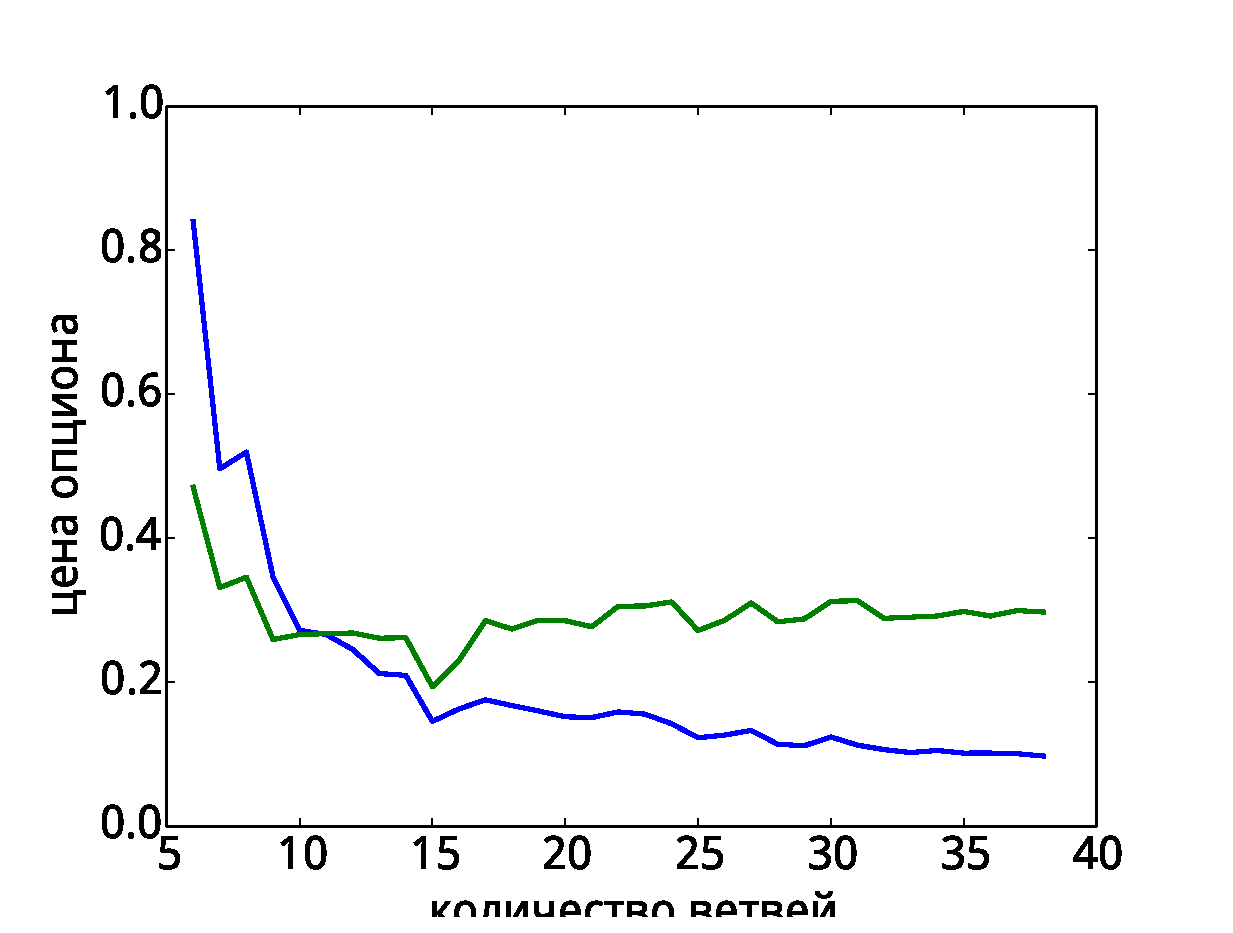
\includegraphics[width=0.8\textwidth]{true_value_test_empiric_distr}
    		\caption{Верхняя и нижняя оценки стоимости опциона по дереву с анализом эмпирической функцией распределения}
    		\label{fig:true_value_test_empiric_distr}
    		\footnotesize{Оценки стоимости опциона с начальной ценой 100, выписанного на срок 1 год на базовый актив с риск-нейтральной процентной ставкой $r = 0.05$, дивидендной ставкой $\delta = 0.1$ и волатильностью $\sigma=0.2$, цена которого --- случайный процесс, являющийся геометрическим броуновским движением с параметрами $\mu = r - \delta$ и $\sigma$, исполняемого 4 раза в году}
	    \end{figure}
		Из графика видно, что сходимости к истинному значению не наблюдается.
\section{Конечная сетка состояний}
	    \subsection{Описание метода}
	        Для того, чтобы сложность алгоритма по  памяти составляла $O(bm)$, необходимо начиная с некоторого момента ограничивать множество состояний, в которые может перейти актив из данного. Так как мы имеем дело с нестационарным случайным процессом, распределение состояний на следующем шаге меняется, как только мы получаем новую реализацию состояния на предыдущем шаге.

	        Можно использовать знания о законе распределения, которому подчиняется состояние базового актива, чтобы уменьшить число возможных состояний.
	        $$dS_t = \mu S_t dt + \sigma S_t dW_t \implies \log \left(\frac{S_t}{S_0}\right)\sim N\left(\left(\mu - \frac{\sigma^2}{2}\right)t, \sigma^2 t\right).$$
	        Ограничив множество состояний базового актива в момент времени $t$ числом $n$, мы можем рассчитать, попадание в какие $n$ классов состояний будет равновероятно. Пусть $F(x)$ --- функция распределения $N\left(0, 1\right)$, тогда
	        \begin{align}
	            \forall i \in 1:n \;\;\exists\; \xi_i = F^{-1}\left(\frac{i-0.5}{n}\right) \text{ --- представитель $i$-го состояния} ,\\
	            \forall i \in 0:n \;\;\exists\; z_i = F^{-1}\left(\frac{i}{n}\right) \text{ --- граница $i$-го состояния} .
	        \end{align}
	        Для каждого момента времени $t_i$ определено множество состояний $$S_i^j = S_0\exp\left(\left(\mu - \frac{\sigma^2}{2}\right)t + \sigma \sqrt{t}\xi_j\right), j\in 1:n$$ и множество границ этих состояний $$Z_i^j = S_0\exp\left(\left(\mu - \frac{\sigma^2}{2}\right)t + \sigma \sqrt{t}z_j\right), j\in 1:n.$$
	        Для любого состояния $S_i^{j_1\cdots j_i}$ найдётся $k\in 1:n : Z_i^{k-1} \leq S_i^{j_1\cdots j_i} < Z_i^k$, тогда $S_i^{j_1\cdots j_i} := S_i^j$. Иллюстрация процесса --- на рис.\ref{fig:grid}
	        \begin{figure}[h]
        	    \centering
        		\caption{Дискретизация по квантилям $GBM(\mu, \sigma)$}
        		\label{fig:grid}
        	\end{figure}
	        Множество состояний не зависит от имеющихся результатов моделирования, только от параметров базового актива, следовательно, генерируемые траектории будут достаточно независимы, чтобы подходить под условия сходимости оценок \eqref{eq:upper}, \eqref{eq:lower}. Количество возможных состояний на каждом шаге можно увеличивать по мере увеличения $t_i$, что может частично компенсировать растущую дисперсию.
	        \subsection{Численные результаты}
	            Результаты моделирования для оценки стоимости того же опциона, что был использован для демонстрации классического алгоритма, представлены на рис. \ref{fig:true_value_test_finite_grid}
                \begin{figure}[h]
                    \centering
                    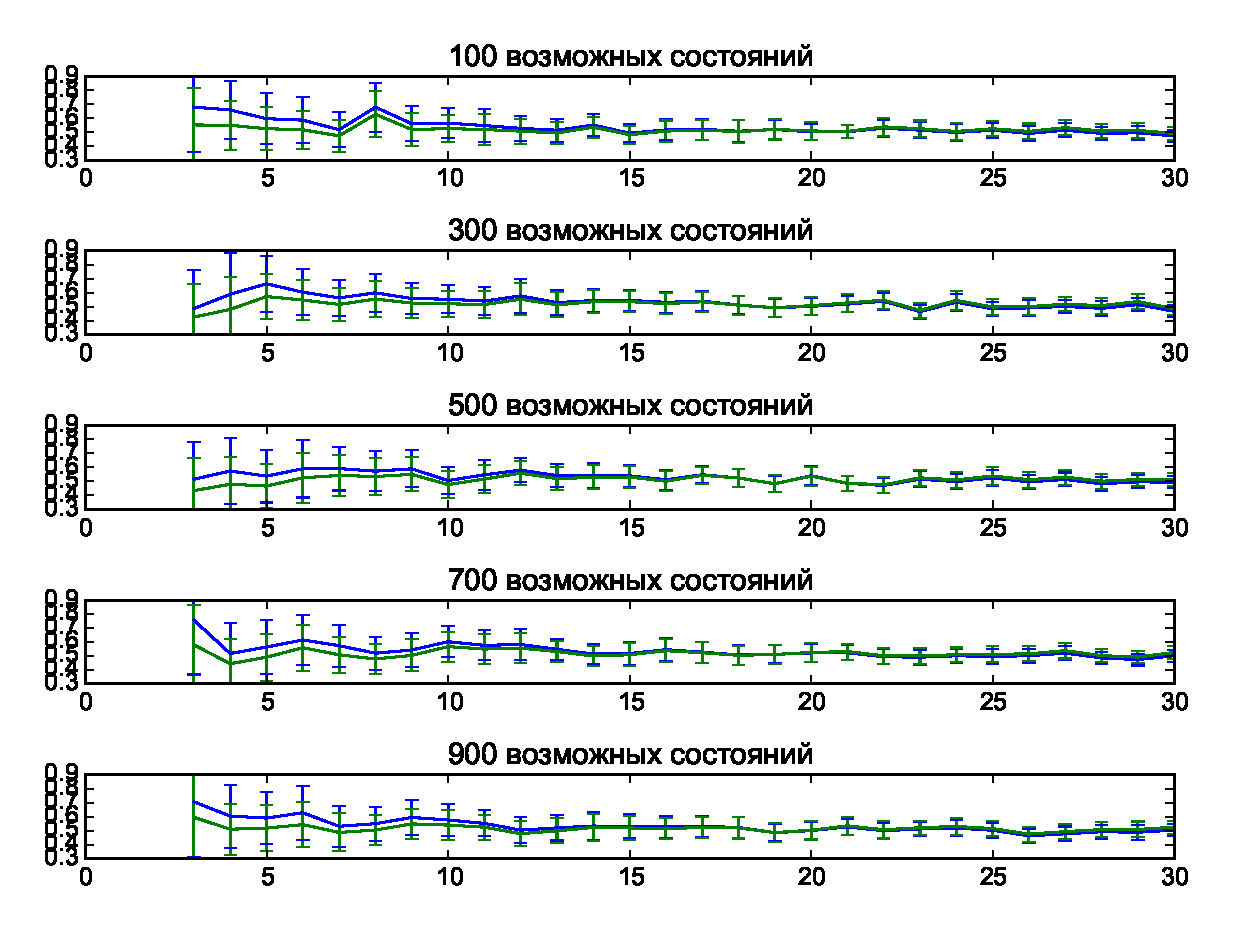
\includegraphics[width=\textwidth]{true_value_test_finite_grid}
                    \caption{Верхняя и нижняя оценки стоимости опциона по дереву с анализом эмпирической функцией распределения}
                    \label{fig:true_value_test_finite_grid}
                    \footnotesize{Оценки стоимости опциона с начальной ценой 100, выписанного на срок 1 год на базовый актив с риск-нейтральной процентной ставкой $r = 0.05$, дивидендной ставкой $\delta = 0.1$ и волатильностью $\sigma=0.2$, цена которого --- случайный процесс, являющийся геометрическим броуновским движением с параметрами $\mu = r - \delta$ и $\sigma$, исполняемого 4 раза в году}
                \end{figure}
                Несмотря на выполнение условий сходимости, налагаемых на траектории, вычисления демонстрируют отсутствие сходимости при $b \to \infty$: при больших значениях $b$ ($b=60, 80$, не показаны на графике) оценки демонстрируют устойчивое поведение, и среднее значение верхней и нижней оценки по 100 реализаций для каждого $b$ равны $0.48\pm 0.02$ и $0.43\pm 0.03$ соответственно.
\conclusion

В работе были рассмотрены оценки стоимости американского опциона, которые строятся на базе имитационных моделей. Эти оценки требуют экспоненциально растущей с ростом времени вычислительной работы, и для преодоления этого препятствия была использована идея рандомизации. При этом была использована аналогия, возникающая между методами динамического программирования, используемыми при построении оценок американского опциона, и методами решения интегральных уравнений с полиномиальной нелинейностью.

Алгоритмы, предложенные в главах 2 и 3, реализованы, и с их помощью на вычислительных примерах показано, что соответствующее <<проклятье размерности>> может быть преодолено с помощью подбора соответствующих констант вероятности обрыва траектории. Таким образом, получен новый результат относительно возможности приближённой оценки без экспоненциального роста вычислительной работы.
\nocite{*}
\bibliographystyle{ugost2008}
\bibliography{biblio-u}
\end{document}